%傅里叶级数(三角)

% 未完成: 感觉函数基底需要一些图.
% 如果只考虑某个区间的展开, 不需要使用周期性, 也可以只用 sin 展开, 例如无限深势阱. 现在在考虑要不要先介绍这个呢?? 毕竟量子力学中使用得非常多.
% 仍然用几何矢量来推导!因为怎么可能不会几何矢量就来学高数!
% 注意给出的函数基底正交并不归一!不要改成归一,尽量和《高数》课本一致吧!
% 提一下,我们也可以先把基底正交归一化,最后就不用除以模长了.

% 未完成,应该提一提 delta 符号

\pentry{几何矢量,定积分\upref{DefInt}}% 链接未完成

\subsection{结论}
满足\textbf{狄利克雷条件}的周期函数 $f(x)$ (周期为 $2l$ )可以使用以下三角函数展开
\begin{equation}\label{FSTri_eq1}
f( x ) = \frac{a_0}{2} + \sum\limits_{n = 1}^\infty {{a_n}\cos (\frac{n\pi}{l}x) + } \sum\limits_{n = 1}^\infty {{b_n}\sin (\frac{n\pi}{l}x)}
\end{equation}
其中
\begin{equation}\label{FSTri_eq2}
{a_n} = \frac{1}{l}\int_{ - l}^l {f( x )\cos (\frac{n\pi}{l}x)\D x} 
\end{equation}
\begin{equation}\label{FSTri_eq3}
{b_n} = \frac{1}{l}\int_{ - l}^l {f( x )\sin (\frac{n\pi}{l}x)\D x}
\end{equation}
狄利克雷条件:函数值有限,存在有限个间断点和有限个极值点.

\subsection{说明}
注意\autoref{FSTri_eq1} 的所有 $a_n$ 项为偶函数项,所有 $b_n$ 项为奇函数项.若 $f(x)$ 是偶函数,所有 $b_n$ 项为零,若是奇函数,则所有 $a_n$ 项为零\footnote{证明:如果 $f(x)$ 是偶函数,那么 \autoref{FSTri_eq3} 中的被积函数就是奇函数,所以在区间 $[-l,l]$ 的积分为零.奇函数的证明类似.}. 如果 $f(x)$ 不具有奇偶性,可以表示为偶函数和奇函数之和,分别对应所有 $a_n$ 项和所有 $b_n$ 项
\begin{equation}
f(x) = \frac 12 [f(x)+f(-x)] + \frac 12 [f(x)-f(-x)]
\end{equation}

$f(x)$ 的函数值既可以是实数也可以是复数.实函数的展开系数 $a_n, b_n$ 也必须取实数,复函数的展开系一定不全是实数.

\subsection{完备性}
傅里叶级数最奇妙的地方大概就是它能展开任意满足狄利克雷条件的函数,这个性质叫做\textbf{完备性}.一般高等数学教材中不证明完备性,这里只给出几个例子说明随着求和项数增加,三角函数如何逼近不连续或不光滑的函数.

% 未完成:怎样能实现例子的 environment 呢?
% 1.要求标题左对齐,加粗
% 2.要求环境内用不同的字体,包括公式,稍小

\begin{exam}{方波}

首先定义一个方波为
\begin{equation}
f(x) = \left\{ \begin{aligned}
1& \quad && 2k\pi < x \le (2k + 1)\pi \\
- 1& &&   (2k - 1)\pi < x \le 2k\pi 
\end{aligned}\right.
\end{equation}
注意 $f(x)$ 在 $x=k\pi$ 处存在间断点.进行傅里叶级数展开得
\begin{equation}
f(x) = \sum\limits_{k = 0}^{ + \infty } {\frac{4}{{\pi (2k + 1)}}\sin (2k + 1)x}
\end{equation}
注意由于 $f(x)$ 是奇函数,求和只有正弦项.取级数的前 $m$ 项求和并画图如\autoref{FSTri_fig1}.

\begin{figure}[ht]
\centering
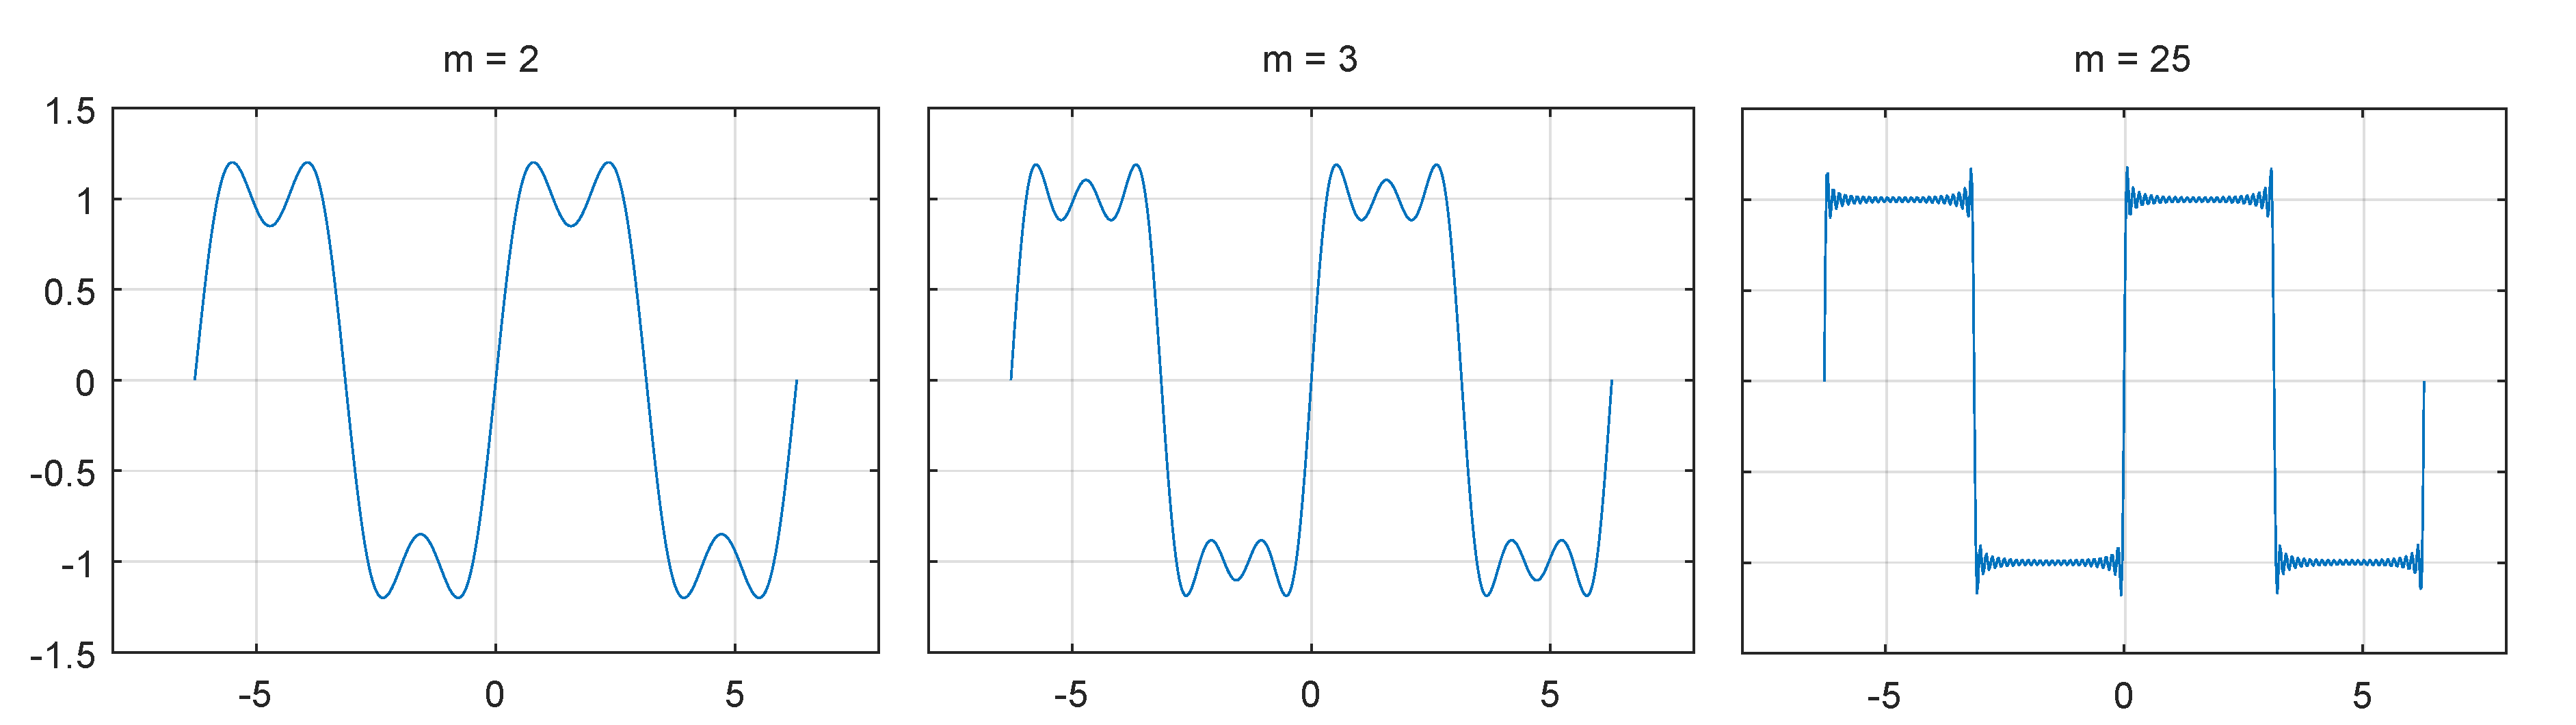
\includegraphics[width=14.5cm]{./figures/FSTri1.pdf}
\caption{有限项傅里叶级数逼近方波}\label{FSTri_fig1}
\end{figure}
\end{exam}

\begin{exam}{正弦函数的绝对值} % 未完成:图

偶函数 $f(x) = \abs{\sin x}$ 存在不光滑的点,展开成傅里叶级数为
\begin{equation}
f(x) = \abs{\sin x} = \frac{2}{\pi } - \frac{4}{\pi }\sum\limits_{k = 1}^{ + \infty } {\frac{1}{{4{k^2} - 1}}\cos 2k} x
\end{equation}
前 $m$ 项和画图如\autoref{FSTri_fig2}.
\begin{figure}[ht]
\centering
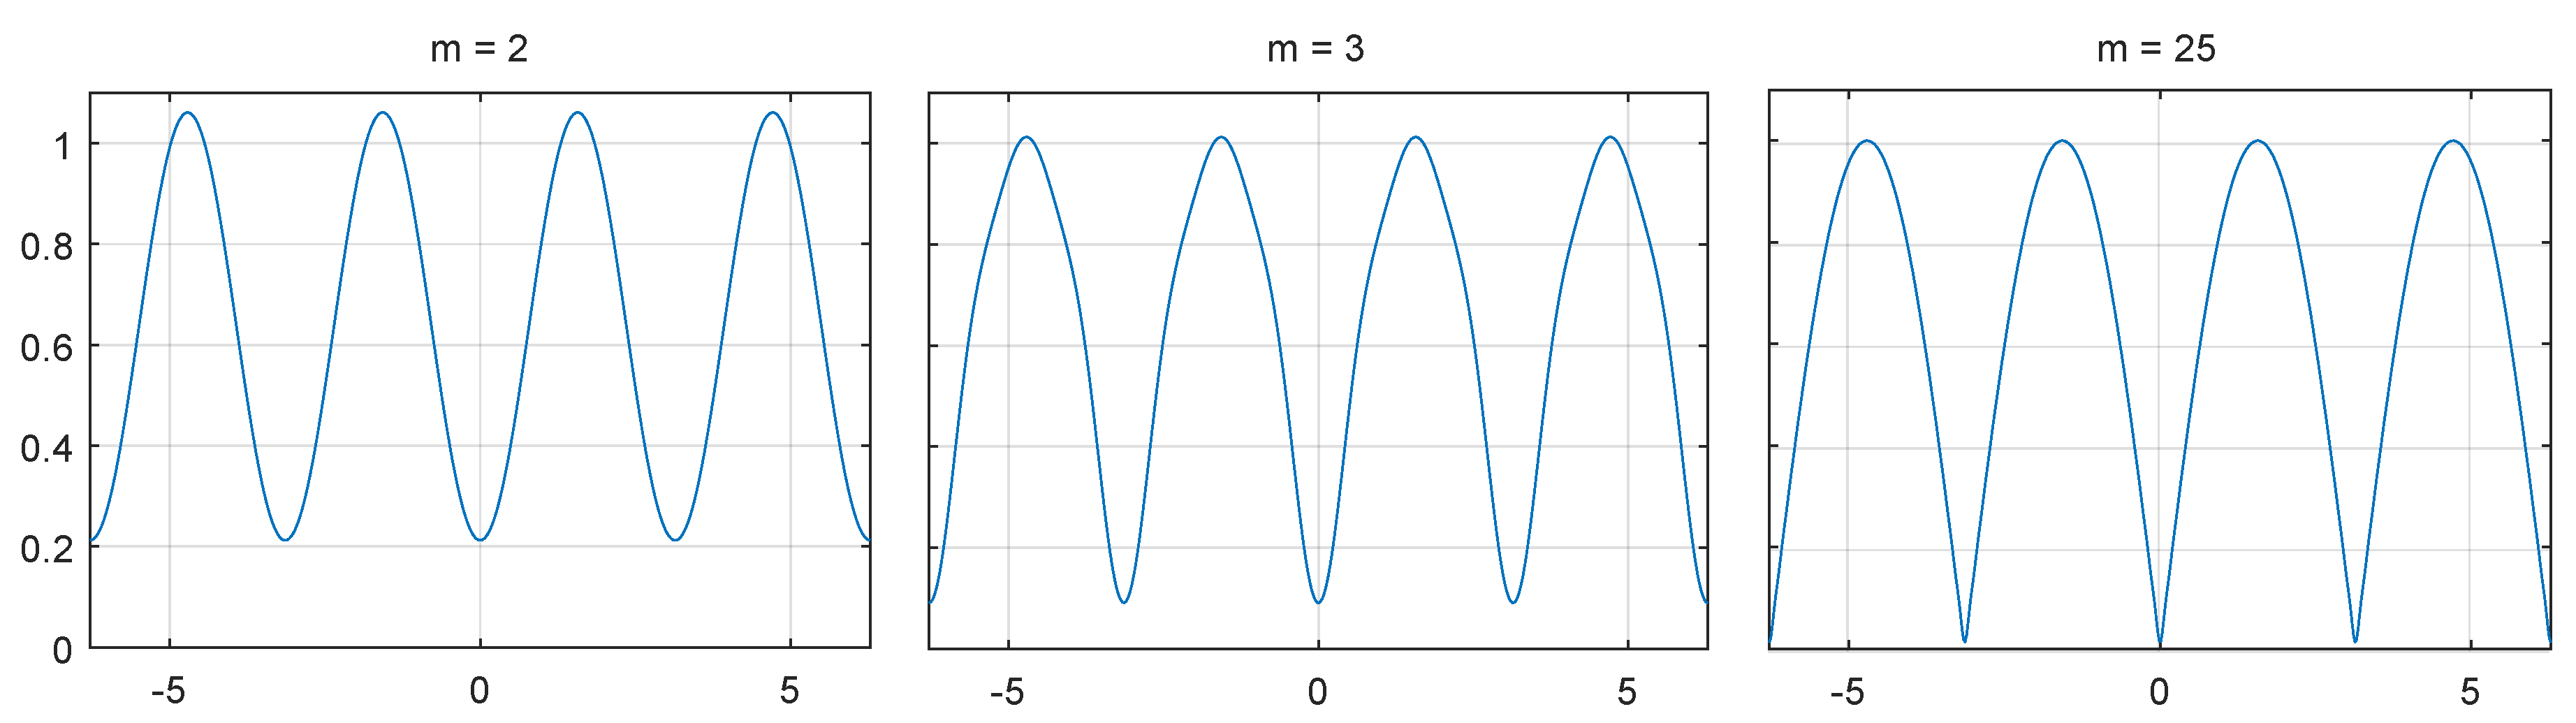
\includegraphics[width=14.5cm]{./figures/FSTri2.pdf}
\caption{有限项傅里叶级数逼近 $\abs{\sin(x)}$}\label{FSTri_fig2}
\end{figure}
\end{exam}


\subsection{系数公式推导}
% 还是用矢量公式比较好

在泰勒级数\upref{Taylor} 中,% 链接未完成
我们通过求 $n$ 阶导数的方式来“过滤”出第 $n$ 阶系数.这里我们用积分的方式来“ 过滤” 系数.这里我们通过一个重要的类比来讲解,即几何矢量在正交(不归一)基底上的展开.% 链接未完成

% 感觉先上图最容易懂. 还是先说 sin&cos 基底再介绍单独的 sin 基底 (注意包括 “1”)(cos 基底提一下就好), 用于某个区间内的函数,不需要拓展成周期函数的情况.
% 

给出一组无穷多个函数
\begin{equation}\label{FSTri_eq4}
\frac 12,\;   \sin\frac{\pi}{l} x,\;   \cos\frac{\pi}{l} x,\;   \sin\frac{2\pi}{l} x,\;   \cos\frac{2\pi}{l} x,\;   \dots\;\sin\frac{n\pi}{l} x,\;   \cos\frac{n\pi}{l} x\;   \dots
\end{equation}
其中 $n$ 是正整数.我们把任意满足狄利克雷条件的函数(以下简称任意函数)比作几何矢量,把上面这组函数(\autoref{FSTri_eq4})比作矢量基底(称为\textbf{函数基底})
,任意函数都可以表示成这组基底的线性组合(\autoref{FSTri_eq1}).现在把两个任意函数(矢量) $f(x)$ 和 $g(x)$ 的\textbf{点乘}定义为它们的乘积在 $[-l,l]$ 内积分
\begin{equation}
\bra{f}\ket{g} = \int_{-l}^{l} f(x)g(x)\D x
\end{equation}
可以证明这组基底\textbf{正交}(即任意两个不同的基底点乘为 0,证明见词条最后)但不\textbf{归一}(某矢量与自身点乘等于 1).与“几何矢量在正交但不归一的基底上展开”一样,我们只要把函数分别与各个基底点乘,再除以基底的模长平方(模方)
即可获得线性组合的系数 $a_n$ 和 $b_n$. 可以证明所有基底的模方为 $l$, 这样我们就得到了系数公式(\autoref{FSTri_eq2} \autoref{FSTri_eq3}).


\subsection{正弦基底}
若我们只需要在一个区间 $[0,l]$ 上展开函数 $f(x)$ 而不在意其他地方,那么我们可以假想 $f(x)$ 是以 $2l$ 为周期的奇函数,这样,我们只需要用正弦基底展开 $f(x)$ 即可\footnote{显然我们也可以假想 $f(x)$ 是以 $2l$ 为周期的偶函数,用余弦基底展开 $f(x)$.但更常见的是使用正弦基底,经常在量子力学中使用,因为无限深势阱要求波函数在区间两端消失.}. 于是我们可以说,\autoref{FSTri_eq4} 中给出的所有正弦基底在区间 $[0,l]$ 具有完备性.

\begin{exam}{用正弦基底展开闭区间内的函数}

定义区间 $[0,a]$ 内的一个三角形函数如下,先把函数归一化,再用正弦基底做傅里叶展开.
\begin{equation}
f(x) = 
\left\{\begin{aligned}
&\frac 2a x &\quad (0 < x \le \frac a2)\\
&2 -\frac 2a x &\quad (\frac a2 < x < a)
\end{aligned}\right.
\end{equation}
% 未完成:分段函数图

首先假想 $f(x)$ 为奇函数,原则上可以直接使用\autoref{FSTri_eq3} 计算展开系数,但由于被积函数 $f(x)\sin(x)$ 为偶函数, 可以先把\autoref{FSTri_eq3} 化简为%未完成:介绍定积分的时候也讲讲偶函数奇函数的化简呗
\begin{equation}
{b_n} = \frac{2}{a}\int_{0}^a {f( x )\sin (\frac{n\pi}{a}x)\D x}
\end{equation}

% 未完成: 对称性图,同时画出函数和基底

又注意 $f(x)$ 关于区间中点的对称性,我们可以进一步判断出(如图*) $n$ 为偶数时 $b_n$ 项都为零, 而 $n$ 为奇数项的 $b_n$ 在 $[0,a/2]$ 的积分等于在 $[a/2,a]$ 的积分, 所以
\begin{equation}\begin{aligned}
{b_n} &= \frac{4}{a}\int_{0}^{a/2} {f( x )\sin (\frac{n\pi}{a}x)\D x}\\
&= \frac{8}{a^2} \int_{0}^{a/2} {x\sin (\frac{n\pi}{a}x)\D x}
\end{aligned}\end{equation}
这个积分既可以见例*%未完成:例子放到分部积分里面吧
,也可以用 Wolfram Alpha 或 Mathematica 完成.%未完成:链接
结果是
\begin{equation}
b_n = (-1)^{\frac{n-1}{2}} \frac{8}{\pi^2 n^2} \quad (n\text{为奇数})
\end{equation}

\end{exam}

进一步说,我们可以用正弦基底在任意区间 $[x_0,x_0+l]$ 上展开任意函数.要这样做,我们只需要把所有正弦基底平移 $x_0$ 即可.
\begin{equation}
\sin\frac{\pi}{l} (x-x_0),\;   \sin\frac{2\pi}{l} (x-x_0),\;    \dots\;\sin\frac{n\pi}{l} (x-x_0) \dots
\end{equation}

% \subsection{使用归一化的基底}
% 未完成:我们也可以把基底归一化,这样的好处就是,系数模方之和会等于被展开函数的模方.这个“归一化不变”的特点可以拓展到傅里叶变换中,直接导致了归一化系数 sqrt(2pi) 的出现.

\subsection{证明函数基底正交}
% 未完成:需要拓展到 2l 区间!

现在证明任意两个不同的基底点乘等于 0.当$m \ne n$时,有
\begin{equation}\begin{aligned}
&\int_{ - \pi }^\pi  {\sin(mx) \vdot \sin(nx) \D x} \\
 = &\frac{1}{2}\int_{ - \pi }^\pi  {\cos [ {(m - n)x} ]\D x}  - \frac{1}{2}\int_{ - \pi }^\pi  {\cos [ {(m + n)x} ]\D x}  = 0
\end{aligned}\end{equation}

\begin{equation}\begin{aligned}
&\int_{ - \pi }^\pi  {\cos(mx) \vdot \cos(nx) \D x} \\
 =  &- \frac{1}{2}\int_{ - \pi }^\pi  {\cos [ {(m - n)x} ]\D x}  + \frac{1}{2}\int_{ - \pi }^\pi  {\cos [ {(m + n)x} ]\D x}  = 0
\end{aligned}\end{equation}

\begin{equation}\begin{aligned}
&\int_{ - \pi }^\pi  {\sin(mx) \vdot \cos(nx) \D x}\\
= &\frac{1}{2}\int_{ - \pi }^\pi  {\sin [ {(m + n)x} ]\D x}  - \frac{1}{2}\int_{ - \pi }^\pi  {\sin [ {(m - n)x} ]\D x} = 0
\end{aligned}\end{equation}

\begin{equation}
\int_{ - \pi }^\pi  {1 \vdot \sin x \D x}  = 0
\end{equation}

\begin{equation}
\int_{ - \pi }^\pi  {1 \vdot \cos x \D x}  = 0\\
\end{equation}
其中任意一个函数与自己点乘都等于$\pi $ (除了常函数1积分为 $2\pi$).
\begin{equation}
\int_{ - \pi }^\pi {{{\sin }^2}(nx) \D x} = \pi
\end{equation}
\begin{equation}
\int_{ - \pi }^\pi {{{\cos }^2}(nx) \D x} = \pi
\end{equation}
\begin{equation}
\int_{ - \pi }^\pi {{1^2}\D x} = 2\pi
\end{equation}

